\documentclass[letterpaper, 12pt]{article}
\usepackage[top=2cm,bottom=1cm,left=0.75in,right=0.75in,headheight=17pt, % as per the warning by fancyhdr
includehead,includefoot,
heightrounded, % to avoid spurious underfull messages
]{geometry}
\addtolength{\topmargin}{-.25in}
\usepackage{fancyhdr}
\pagestyle{fancy}
\usepackage{graphicx}
\usepackage{lastpage}
\usepackage{gensymb}

\begin{document}
\fancyhead[l]{	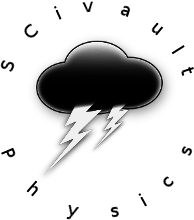
\includegraphics[height=1.2cm]{../Logo/sp.png} Name:}
\fancyhead[r]{REFERENCE MATERIAL}
\cfoot{\thepage\ of \pageref{LastPage}}
	


\begin{center}Things to Memorize: Waves
\end{center}

\subsection*{Types of Waves}
	\begin{itemize}
		\item \textbf{Longitudinal Waves} - Are waves in which the displacement is perpendicular to the direction of travel.  (like an ocean wave)
		
		\item \textbf{Transverse Waves} - Are waves in which the displacement is along the same axis as the direction of travel.  (Like a Sound Wave or a shock wave)
		\item \textbf{Electromagentic Waves} - are all forms of light (both visible and invisible)
	\end{itemize}
\subsection*{Wave Measurements}
	\begin{itemize}
		\item \textbf{Crest}s are the highest points on a wave.
		\item \textbf{Trough}s are the lowest points on a wave. 
		\item \textbf{Amplitude} - How big or strong a wave is.  Measured from center to crest or center to trough.  
		\begin{itemize}
			\item We see the amplitude of visible light as \textbf{brightness}.
			\item We hear the amplitude of a sound wave as \textbf{volume} (loudness). 
		\end{itemize}
		\item \textbf{Wavelength} - The distance (in meters) from one point on a wave to an identical point on the wave.  
		\item \textbf{Period} - The time it takes a wave to repeat itself. 
		\item \textbf{Frequency} - How many times a wave repeats itself in one second. 
		\begin{itemize}
			\item We see the frequency of a light wave as \textbf{color}.
			\item We hear the frequency of a sound wave as \textbf{pitch}. 
		\end{itemize}
	\end{itemize}
\newpage 
\subsection*{Wave Phenomena}
	\begin{itemize}
		\item \textbf{Interference} - Two waves overlap.
		\begin{itemize}
			\item If they make a bigger wave, it is \textbf{constructive} interference. 
			\item If they make a smaller wave, it is \textbf{destructive} interference. 
		\end{itemize}

		\item \textbf{Resonance} - one wave creates a similar wave in a nearby object. (Like when a saxaphone plays a note, the snare drum starts to vibrate).
		\item \textbf{Doppler Effect} - The frequency of a wave seems to change due to the motion of the source and the observer. 
			\begin{itemize}
				\item When they move toward each other, a higher pitch is observed.
				\item When they move away from each other, a lower pitch is observed.
			\end{itemize}
		\item \textbf{Refraction} - A wave changes direction due to a change in \textbf{medium}.
		\item \textbf{Diffraction} - A wave changes direction due to interaction with a sharp edge of an object. 
		\item \textbf{Polarization} - The direction that a wave is vibrating. 
	\end{itemize}
	

 




\end{document}
